\chapter[Revisão Estruturada da Literatura]{Revisão Estruturada da Literatura}
\label{cap:revisao}

Este capítulo tem como objetivo expor o protocolo usado para filtrar, selecionar, extrair e analisar os dados necessários para responder às questões de pesquisa deste estudo. Também são apresentados a condução da busca e os resultados levantados. A busca foi realizada na base Scopus \cite{elsevier2026}, por indexar publicações de diversas editoras da área de engenharia de software e permitir buscas estruturadas, o que contribui para manter o rigor da revisão.

\section{Protocolo}
\label{sec:protocolo}

O protocolo utilizado foi estruturado com base no modelo de revisão sistemática da literatura de \citeonline{kitchenham2007}. O registro prévio dos métodos reduz o viés dos pesquisadores e permite replicar e auditar o estudo, de modo que a aplicação do mesmo protocolo tenda a levar a resultados muito próximos.

\subsection{Questões de pesquisa}
\label{sec:qps}

A Tabela~\ref{tab:qps} apresenta as questões secundárias de pesquisa que a revisão busca responder.

\begin{table}[H]
  \centering
  \caption{Questões secundárias de pesquisa}
  \label{tab:qps}
  \small
  \begin{tabular}{|p{0.1\textwidth}|p{0.8\textwidth}|}
    \hline
    \textbf{QP} & \textbf{Descrição} \\ \hline
    QP1 & Quantos estudos foram publicados por ano do total selecionado? \\ \hline
    QP2 & Em que veículos os estudos foram publicados e em que contexto foram conduzidos? \\ \hline
    QP3 & Que tipos de estudo empírico são adotados? \\ \hline
    QP4 & Quais modelos de linguagem são mais utilizados na geração de critérios de aceitação? \\ \hline
    QP5 & Quais técnicas são mais empregadas para apoiar a geração? \\ \hline
    QP6 & Quais artefatos são fornecidos como entrada? \\ \hline
    QP7 & Quais mecanismos automáticos de verificação ou refinamento dos critérios gerados? \\ \hline
    QP8 & Quais métricas de avaliação são mais comumente usadas para avaliar os critérios de aceitação gerados? \\ \hline
    QP9 & Quais limitações e desafios são mais relatados nos estudos sobre geração de critérios de aceitação com LLMs? \\ \hline
  \end{tabular}
  \fonte{Autores}
\end{table}

\subsection{\textit{String} de busca}
\label{sec:string}

A busca em bases acadêmicas exige uma estratégia definida, pois uma \textit{string} mal construída pode retornar muitos estudos sem relação com o tema ou poucos estudos para responder às questões de pesquisa.

O escopo da revisão foi delimitado com a estrutura PICOC \cite{kitchenham2007}, derivada do PICO, usado na área da medicina \cite{pai2004}. A \textit{string} de busca foi construída a partir de três desses elementos: \textbf{População}, \textbf{Intervenção} e \textbf{Resultado}, conforme a Tabela~\ref{tab:picoc}. A \textbf{Comparação} não foi incluída por se tratar de uma revisão de caracterização, e o \textbf{Contexto} foi aplicado apenas pelo período, restrito a publicações a partir de 2022 (PUBYEAR $>$ 2021). A Figura~\ref{fig:estrategia-busca} ilustra a estratégia de busca.

\begin{figure}[H]
  \centering
  \caption{Uma visão geral da estratégia de busca na literatura}
  \label{fig:estrategia-busca}
  
\includegraphics[width=0.6\textwidth]{figuras/estrategia-busca-pico.png}
  \fonte{Adaptado de \citeonline{pai2004}}
\end{figure}

Como o PICO tem origem na medicina, seus elementos precisaram ser interpretados para o contexto da engenharia de software. A \textbf{População} passa a representar a área de aplicação, e a \textbf{Intervenção}, as abordagens baseadas em LLMs, incluindo técnicas de \textit{prompting} e entradas multimodais. O \textbf{Resultado} corresponde aos CA e às formas como eles aparecem nos estudos, como histórias de usuário e cenários em \textit{Gherkin}. A Tabela~\ref{tab:picoc} apresenta o termo central de cada elemento e seus termos relacionados.

\begin{table}[H]
  \centering
  \caption{Elementos do PICOC usados na \textit{string} de busca}
  \label{tab:picoc}
  \small
  \begin{tabular}{|p{0.15\textwidth}|p{0.2\textwidth}|p{0.55\textwidth}|}
    \hline
    \textbf{Elemento} & \textbf{Termo central} & \textbf{Sinônimos e termos relacionados} \\ \hline
    \textbf{População} & \textit{Software engineering} & \textit{software, agile} \\ \hline
    \textbf{Intervenção} & \textit{Large language models} & \textit{large language model, LLM, LLMs, generative AI, generative artificial intelligence, ChatGPT, GPT-4, Copilot, multimodal, multi-modal, language models, claude, gemini, llama, prompt, deepseek, qwen, kimi, grok} \\ \hline
    \textbf{Resultado} & \textit{Acceptance criteria} & \textit{acceptance criteria, acceptance criterion, user story, user stories, Gherkin, behavior-driven development, BDD, acceptance test, test scenarios} \\ \hline
  \end{tabular}
  \fonte{Autores}
\end{table}

Os termos de cada bloco foram combinados com o operador OR, e os blocos, com o operador AND, de modo a recuperar os estudos situados na interseção dos blocos, como ilustra a Figura~\ref{fig:estrategia-busca} \cite{pai2004}.

A \textit{string} foi aplicada a título, resumo e palavras-chave (TITLE-ABS-KEY). O bloco de Intervenção inclui nomes de modelos, pois parte dos estudos cita o produto utilizado, como o ChatGPT, em vez de termos gerais como LLM. O bloco de \textbf{Resultado} inclui termos sobre histórias de usuário e testes de aceitação, pois os CA costumam aparecer como parte desses artefatos, e não como objeto principal do estudo. A pertinência dos estudos foi verificada depois, nos critérios de elegibilidade. A \textit{string} foi calibrada em testes na Scopus: o bloco de \textbf{Resultado} foi ampliado com os termos \textit{acceptance test} e \textit{test scenarios} para recuperar mais estudos, e o termo \textit{Given-When-Then} foi retirado por não trazer resultados adicionais. A versão final recuperou os dois artigos usados como referência na calibração \cite{ferreira2025,wang2025} e foi executada em 23/09/2026, conforme apresentado a seguir.

\begin{center}
( TITLE-ABS-KEY ( ( "software" OR "agile" ) AND ( "large language model" OR "LLM" OR "LLMs" OR "generative AI" OR "generative artificial intelligence" OR "ChatGPT" OR "GPT-4" OR "Copilot" OR "multimodal" OR "multi-modal" OR "language models" OR "claude" OR "gemini" OR "llama" OR "prompt" OR "deepseek" OR "qwen" OR "kimi" OR "grok" ) AND ( "acceptance criteria" OR "acceptance criterion" OR "user story" OR "user stories" OR "Gherkin" OR "behavior-driven development" OR "BDD" OR "acceptance test" OR "test scenarios" ) ) AND PUBYEAR > 2021 )
\end{center}

\subsection{Critérios de seleção}
\label{sec:criterios}

Após a definição da \textit{string} de busca, foram estabelecidos os critérios de inclusão e exclusão, apresentados na Tabela~\ref{tab:criterios}, com o propósito de selecionar apenas os artigos alinhados ao contexto da pesquisa.

\begin{table}[H]
  \centering
  \caption{Critérios de inclusão e exclusão}
  \label{tab:criterios}
  \small
  \begin{tabular}{|p{0.08\textwidth}|p{0.82\textwidth}|}
    \hline
    \textbf{ID} & \textbf{Critério} \\ \hline
    \multicolumn{2}{|l|}{\textbf{Critérios de inclusão}} \\ \hline
    I1 & O estudo deve utilizar requisitos ou documentação em linguagem natural como entrada, mesmo quando associados a artefatos visuais como telas, protótipos, \textit{mockups} ou código HTML. \\ \hline
    I2 & O estudo deve apresentar avaliação de seus resultados, como a qualidade dos artefatos gerados, o desempenho do modelo na avaliação desses artefatos, utilizando métricas, comparação com uma base de referência ou análise humana. \\ \hline
    I3 & O estudo trata de critérios de aceitação, gerando-os, refinando-os ou avaliando sua qualidade, em qualquer representação, seja como artefato final ou como etapa intermediária do processo. \\ \hline
    I4 & O estudo deve empregar modelos de linguagem de grande porte para gerar, refinar ou avaliar a qualidade de critérios de aceitação. \\ \hline
    \multicolumn{2}{|l|}{\textbf{Critérios de exclusão}} \\ \hline
    E1 & O estudo foi publicado antes de 2022. \\ \hline
    E2 & O estudo não está em inglês ou português. \\ \hline
    E3 & O estudo tem o texto completo indisponível. \\ \hline
    E4 & Estudo duplicado. \\ \hline
    E5 & O estudo consome critérios de aceitação já existentes, fornecidos como entrada e não produzidos pelo próprio estudo, e tem como foco a execução de testes ou a geração de \textit{scripts} executáveis. \\ \hline
    E6 & O estudo utiliza histórias de usuário apenas como entrada para gerar outros artefatos, sem gerar, refinar ou avaliar a própria história ou seus critérios de aceitação. \\ \hline
  \end{tabular}
  \fonte{Autores}
\end{table}
% Os IDs I1-I4 e E1-E6 seguem a ordem do doc; o texto cita I2 e I3 com esse sentido. Conferir com o protocolo do Evidentia.

\subsection{Extração e síntese dos dados}
\label{sec:extracao}

Os dados dos artigos selecionados foram extraídos com o formulário da Tabela~\ref{tab:formulario}, para análise e resposta às questões secundárias de pesquisa.

\begin{table}[H]
  \centering
  \caption{Formulário de extração de dados}
  \label{tab:formulario}
  \small
  \begin{tabular}{|p{0.43\textwidth}|p{0.43\textwidth}|}
    \hline
    \multicolumn{2}{|c|}{\textbf{Campos do formulário}} \\ \hline
    ID & Técnica(s) empregada(s) \\
    Título & Descrição da técnica \\
    Data da extração & Entrada primária \\
    Autores & Artefatos contextuais \\
    Ano de publicação & Forma de fornecimento \\
    Tipo de veículo & Formato de saída \\
    Contexto & Mecanismo de verificação/refinamento \\
    Tipo de estudo (declarado e estratégia empírica) & Referencial de comparação \\
    Participantes & Métricas utilizadas \\
    Modelo(s) de linguagem & Dimensão avaliada \\
    Hospedagem do modelo & Tipo de medida \\
     & Resultados reportados \\
     & Limitações relatadas \\
     & Ameaças à validade \\ \hline
  \end{tabular}
  \fonte{Autores}
\end{table}

A síntese foi predominantemente descritiva e narrativa, complementada por contagens de frequência por ano, veículo, modelo de linguagem, técnica, tipo de entrada e métrica, apresentadas em tabelas e gráficos. Os dados qualitativos, como limitações e desafios, foram agrupados por tema.

Por se tratar de uma revisão estruturada, não foi aplicado um \textit{checklist} formal de avaliação da qualidade dos estudos.

\section{Seleção dos artigos}
\label{sec:selecao}

Para aplicar os critérios de seleção, foram lidos os títulos, os resumos e as palavras-chave de todos os artigos retornados pela \textit{string}, o que resultou na seleção para leitura completa. Por fim, os artigos selecionados foram lidos, e seus dados foram extraídos com o formulário descrito na Seção~\ref{sec:extracao}.

No total, a \textit{string} retornou 287 artigos. Após a remoção de 1 duplicata, 286 foram triados, e 15 foram selecionados para leitura completa. Para complementar esse conjunto, foram incluídos manualmente, por orientação do professor orientador, 11 artigos também retornados pela \textit{string}, mas não selecionados na triagem. Nesses casos, os critérios I3 (tratar de CA) e I2 (avaliar os resultados) foram aplicados de forma restritiva com base no resumo, o que deixou de fora estudos em que os CA aparecem junto com histórias de usuário ou como cenários em \textit{Gherkin}. Foram buscados artigos cujo resumo tratava da geração de CA, de cenários em \textit{Gherkin} ou de histórias de usuário. Nos artigos sobre histórias, o texto completo foi pesquisado com termos ligados a CA (\textit{acceptance criteria}, AC, \textit{acceptance test}). Essa inclusão foi feita porque alguns estudos geram CA junto com as histórias e, mesmo sem tratar apenas de CA, podem responder às questões de pesquisa. Também foram incluídos estudos que geram CA sem avaliá-los formalmente, pois, embora não contribuam para a análise de métricas, ajudam a responder às questões sobre modelos, técnicas e artefatos de entrada.

Após a leitura, 2 artigos foram considerados relatos do mesmo estudo, o que resultou em 25 estudos (26 relatos).

A Tabela~\ref{tab:artigos} lista os artigos selecionados, em que os itens 13 e 18 são relatos do mesmo estudo, e a Figura~\ref{fig:selecao} resume o processo de seleção e a quantidade de artigos em cada etapa.

\begin{small}\begin{SingleSpacing}
\begin{longtable}{|p{0.06\textwidth}|p{0.84\textwidth}|}
  \caption{Artigos selecionados}
  \label{tab:artigos} \\
  \hline
  \textbf{Nº} & \textbf{Título} \\ \hline
  \endfirsthead
  \hline
  \textbf{Nº} & \textbf{Título} \\ \hline
  \endhead
  1 & Empowering Agile-Based Generative Software Development through Human-AI Teamwork \cite{zhang2025} \\ \hline
  2 & Take Loads Off Your Developers: Automated User Story Generation using Large Language Model \cite{rahman2024} \\ \hline
  3 & A design science research approach to Large Language Model-Based Agents for Requirements Specification (LLMBA4RS) in low-code applications \cite{rotar2025} \\ \hline
  4 & Industrial Deployment of an AI Multi-Agent System for Requirements-Driven Code Verification \cite{baker2026} \\ \hline
  5 & From law to Gherkin: A human-centred quasi-experiment on the quality of LLM-generated behavioral specifications from food-safety regulations \cite{hassani2026} \\ \hline
  6 & Multi-Modal Requirements Data-based Acceptance Criteria Generation using LLMs \cite{wang2025} \\ \hline
  7 & SimAC: simulating agile collaboration to generate acceptance criteria in user story elaboration \cite{li2024} \\ \hline
  8 & LLM-Based Agents for Automating the Enhancement of User Story Quality: An Early Report \cite{zhang2024} \\ \hline
  9 & Acceptance Test Generation with Large Language Models: An Industrial Case Study \cite{ferreira2025} \\ \hline
  10 & Automated Assessment and Enhancement of User Story Quality Using Large Language Models in Agile Development \cite{lotfi2025} \\ \hline
  11 & Comparison of Methods for Automated BDD Scenario Generation with NLP and AI \cite{matveeva2025} \\ \hline
  12 & Req2Road: A GenAI Pipeline for SDV Test Artifact Generation and On-Vehicle Execution \cite{zyberaj2026} \\ \hline
  13 & A ChatGPT-powered Prompt Engineering Framework for Generating Software Acceptance Criteria \cite{rawson2025framework} \\ \hline
  14 & From EventStorming Artifacts to User Stories: A Semi-Automated Requirements Extraction Approach \cite{jurgelaitis2026} \\ \hline
  15 & CMAS4G2: A Locally Deployed Cooperative Multi-agent System for Gherkin Acceptance Test Generation \cite{huang2026} \\ \hline
  16 & Comprehensive Evaluation and Insights Into the Use of Large Language Models in the Automation of Behavior-Driven Development Acceptance Test Formulation \cite{karpurapu2024} \\ \hline
  17 & Transforming user story definition: From deterministic to AI-powered automation \cite{avasiloaie2025} \\ \hline
  18 & A ChatGPT-Powered Tool for Automating Context-Aware Acceptance Criteria Generation for User Stories \cite{rawson2025} \\ \hline
  19 & Automated Generation and Refinement of Agile User Stories from Game Design Documents Using Large Language Models \cite{khelifa2026} \\ \hline
  20 & Enhancing Agile Workflows with AI-Driven, Sustainability-Aware Requirements Engineering: A Design Science Approach \cite{weerakoon2026} \\ \hline
  21 & An Analysis of Student Perceptions and Learning Impact of Large Language Models in Requirements Engineering Education \cite{karimi2026} \\ \hline
  22 & From Bugs to Benefits: Improving User Stories by Leveraging Crowd Knowledge with CrUISE-AC \cite{schwedt2025} \\ \hline
  23 & Exploring LLMs Impact on Student-Created User Stories and Acceptance Testing in Software Development \cite{brockenbrough2025} \\ \hline
  24 & Using Generative AI to Create User Stories in the Software Engineering Classroom \cite{brockenbrough2024} \\ \hline
  25 & LLM-Assisted Requirements Engineering in Agile MDD: Industry Insights and Validation \cite{spijkman2025} \\ \hline
  26 & SCLAT: An LLM-Interpretable User Story Quality Evaluation Framework \cite{ma2026} \\ \hline
\end{longtable}
\end{SingleSpacing}\end{small}
\vspace{-0.8\baselineskip}
\fonte{Autores}

\begin{figure}[H]
  \centering
  \caption{Processo de seleção}
  \label{fig:selecao}
  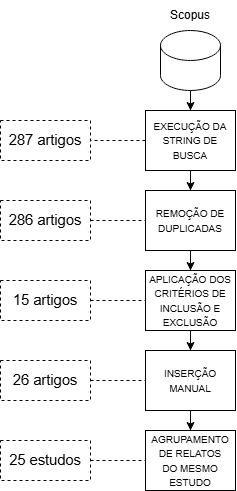
\includegraphics[height=0.55\textheight]{figuras/processo-selecao.png}
  \fonte{Autores}
\end{figure}

\section{Resultados}
\label{sec:resultados-rsl}

Após a leitura dos artigos selecionados, os dados foram extraídos por meio do formulário da plataforma Evidentia Review, utilizada na definição e na execução da revisão por oferecer ferramentas específicas para esse processo. Em seguida, os dados foram organizados em uma \href{https://docs.google.com/spreadsheets/u/0/d/1xJ_K7olUhe2_PlUC02YxyCg5lbETICCPAfx99RQOaOU/edit}{planilha pública}, na qual cada linha representa um artigo e cada coluna, um campo extraído, conforme a Tabela~\ref{tab:formulario}.

As subseções a seguir apresentam os resultados obtidos para as questões secundárias de pesquisa definidas nesta revisão.

% ---------------------------------------------------------------------------
\subsection{QP1 -- Quantos estudos foram publicados por ano do total selecionado?}
\label{sec:qp1}

A Figura~\ref{fig:por-ano} apresenta a distribuição dos 25 estudos incluídos por ano de publicação. Embora a busca abrangesse publicações a partir de 2022, nenhum estudo incluído é de 2022 ou 2023. Os primeiros aparecem em 2024, com 5 estudos (20\%), seguidos de 12 em 2025 (48\%) e 8 em 2026 (32\%). Assim, 80\% dos estudos foram publicados a partir de 2025, o que indica que o tema é recente.

\begin{figure}[H]
  \centering
  \caption{Estudos incluídos por ano de publicação}
  \label{fig:por-ano}
  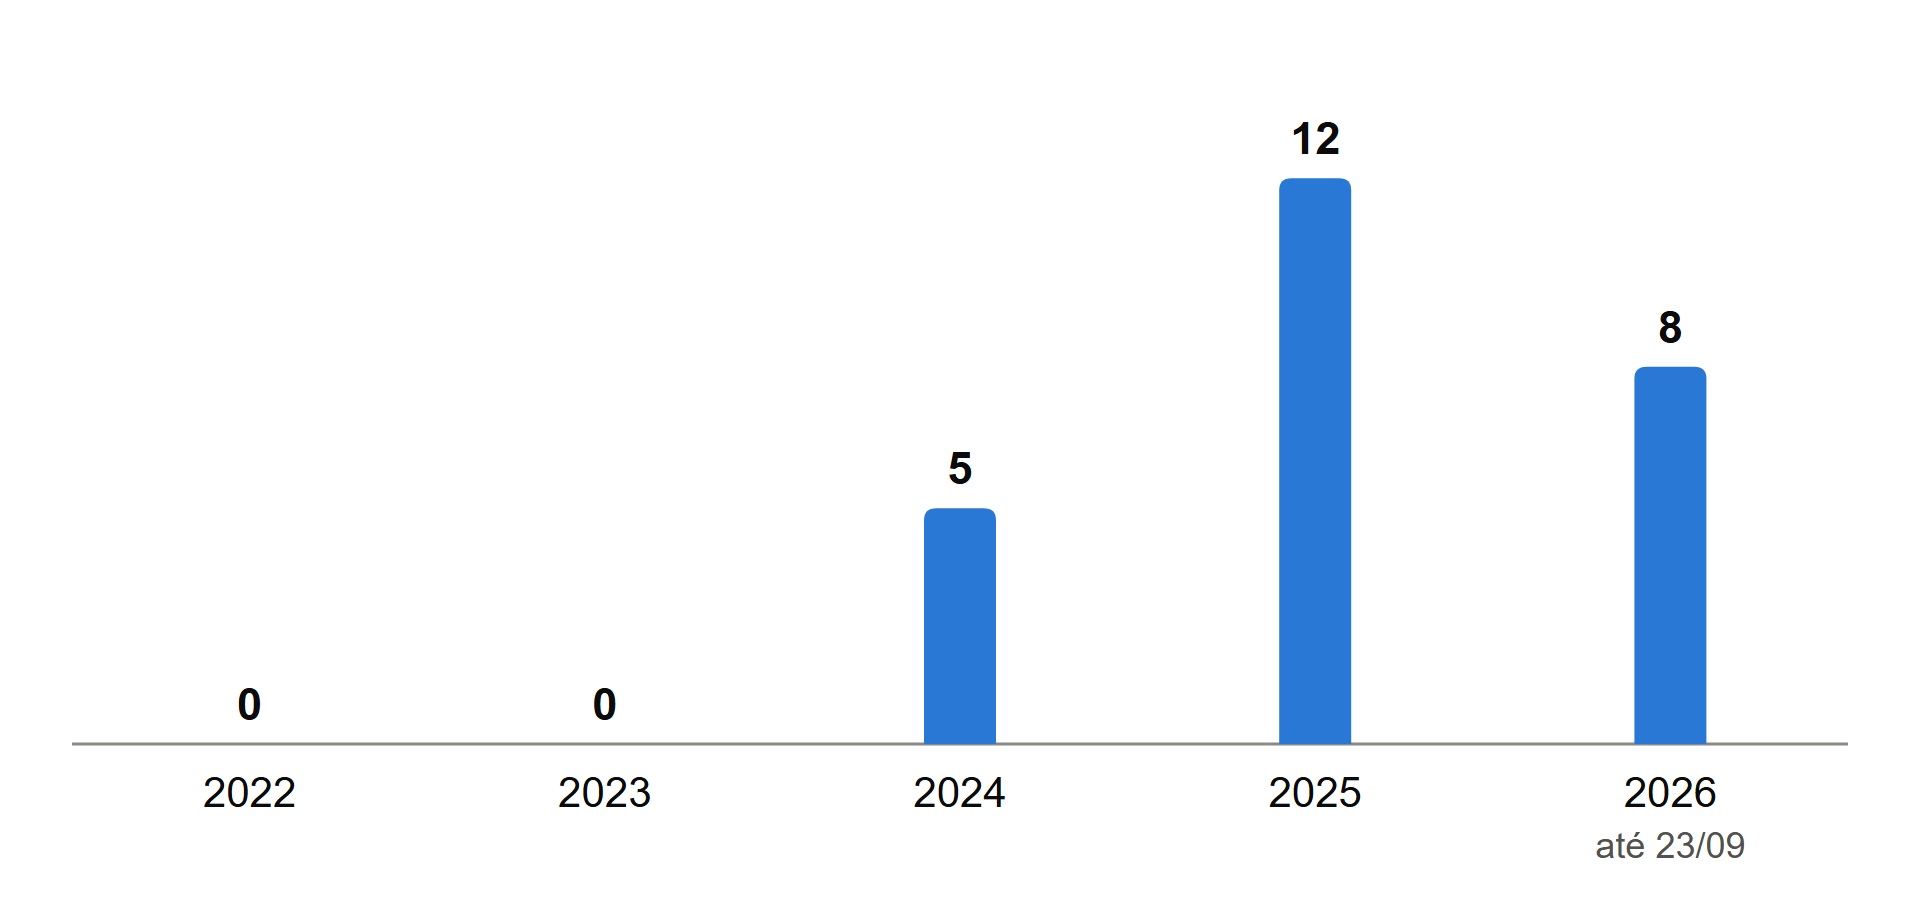
\includegraphics[width=0.7\textwidth]{figuras/estudos-por-ano.png}
  \fonte{Autores}
\end{figure}

O valor de 2026 considera apenas as publicações disponíveis até a execução da busca, em 23/09/2026. Por isso, a diferença em relação a 2025 não indica queda no interesse pelo tema. A distribuição também é coerente com o crescimento observado por \citeonline{cheng2026} na engenharia de requisitos, em que o volume anual de artigos sobre IA generativa passou de 4 em 2022 para 113 em 2024. Na contagem, relatos do mesmo estudo foram considerados uma única vez e, nos artigos de conferência, adotou-se o ano do evento.

% ---------------------------------------------------------------------------
\subsection{QP2 -- Em que veículos os estudos foram publicados e em que contexto foram conduzidos?}
\label{sec:qp2}

Quanto ao veículo, dos 25 estudos incluídos, 16 (64\%) foram publicados em anais de conferências, 7 (28\%) em revistas acadêmicas (periódicos) e 2 (8\%) são \textit{preprints} no arXiv, sem veículo de publicação informado. A predominância de conferências é compatível com o caráter recente do tema, já que esses canais divulgam resultados mais rapidamente do que as revistas.

Quanto ao contexto, os estudos foram classificados pelo ambiente em que foram conduzidos. \citeonline{wohlin2000} caracterizam o contexto de um estudo por dimensões como problema real \textit{versus} problema de brinquedo e profissionais \textit{versus} estudantes. Com base nisso, para definir o contexto, foram observados dois aspectos: a origem dos dados usados como entrada e o perfil de quem avaliou os resultados. Um estudo foi classificado como industrial quando usa dados reais de empresa e é avaliado por profissionais de software ou implantado em produção. Foi classificado como acadêmico quando usa dados públicos, de código aberto, sintéticos ou criados pelos autores e é avaliado por estudantes, pelos próprios autores, por um LLM ou não tem avaliação humana. Os estudos que combinam um aspecto de cada grupo foram classificados como mistos. Dados sintéticos foram tratados como não reais mesmo quando escritos por profissionais de uma empresa ou baseados em um projeto industrial.

Com esse critério, 14 estudos (56\%) foram conduzidos em contexto acadêmico, 6 (24\%) em contexto misto e 5 (20\%) em contexto industrial. Entre os acadêmicos, 8 estudos (32\% do total) não tiveram avaliação humana formal, pois os resultados foram avaliados de forma automática, por um LLM ou apenas pelos próprios autores, e 3 (12\% do total) foram conduzidos em disciplinas, com estudantes como participantes. Nos mistos, a avaliação contou com profissionais, mas os dados eram públicos, adaptados, sintéticos ou de origem não informada. Entre os industriais, 2 estudos (8\%) relatam o uso da solução em produção.

Assim, apenas 5 estudos (20\%) trazem evidências obtidas com dados e profissionais da indústria, enquanto 8 (32\%) não tiveram avaliação humana formal. A maior parte das evidências ainda vem de dados públicos ou criados para o estudo, o que limita a aplicabilidade prática dos resultados na indústria.

% ---------------------------------------------------------------------------
\subsection{QP3 -- Que tipos de estudo empírico são adotados?}
\label{sec:qp3}

Para responder a esta questão, não bastou repetir o que cada artigo diz sobre si mesmo. Os estudos foram classificados pela estratégia empírica que de fato adotam. Um estudo com validação empírica segue um protocolo, o que permite reproduzi-lo, e gera evidência sobre seus resultados, por isso eles são mais confiáveis do que os de um estudo sem essa validação. \citeonline{wohlin2000} descrevem três estratégias empíricas. A \textit{survey} aplica questionários ou entrevistas a uma amostra representativa de uma população definida. O estudo de caso acompanha um projeto ou uma atividade real enquanto ela acontece. Já o experimento exige que os tratamentos sejam atribuídos de forma aleatória, que as hipóteses nula (H0) e alternativa (H1) sejam formuladas ainda no planejamento e que os resultados passem por um teste estatístico; quando não há atribuição aleatória, fala-se em quase-experimento. Abordagens como \textit{design science}, prova de conceito e estudo de viabilidade não aparecem entre essas estratégias, por isso esses estudos foram classificados pela forma como avaliaram seus resultados.

Quando se olha apenas para o que os autores declaram, o experimento é o tipo mais comum, citado por 13 estudos (52\%). Em seguida vêm 4 estudos (16\%) que não nomeiam o método, 3 (12\%) que se apresentam como \textit{design science} e 2 (8\%) como estudo de caso, além de 1 quase-experimento, 1 prova de conceito e 1 estudo de viabilidade. O quadro muda quando os critérios de \citeonline{wohlin2000} são aplicados: apenas 2 estudos (8\%) adotam de fato uma estratégia empírica. Os dois são estudos de caso conduzidos na indústria, um com um sistema implantado em produção \cite{baker2026} e outro com uma ferramenta usada por uma empresa durante dois meses \cite{ferreira2025}. Mesmo nesses casos, os resultados dizem respeito ao contexto observado e são mais difíceis de generalizar do que os de um experimento. Os demais 23 estudos (92\%) não se enquadram em nenhuma das estratégias.

Os motivos variam. A maior parte, 14 estudos (56\%), compara técnicas, modelos ou \textit{prompts}, mas nenhum deles formula H0 e H1 no planejamento, apenas 4 aplicam teste estatístico e só 1 sorteia a distribuição dos participantes entre os tratamentos. O estudo que mais se aproxima de um experimento é um quase-experimento declarado, que compara especificações geradas por dois LLMs e testa estatisticamente a hipótese nula, mas a apresenta apenas na análise dos resultados, sem formulá-la no planejamento nem definir a hipótese alternativa \cite{hassani2026}. Outros 4 (16\%) avaliam as saídas por questionário, mas com pessoas convidadas por conveniência e sem uma população definida, o que não caracteriza uma \textit{survey}. Há ainda 2 estudos (8\%) que se dizem estudos de caso sem acompanhar um projeto em andamento, e 3 (12\%) não medem os resultados com nenhum instrumento definido, como métrica, questionário ou gabarito, limitando-se a exemplos ilustrativos ou a \textit{feedback} informal. Em outras palavras, muitos estudos usam o vocabulário da pesquisa empírica sem adotar o desenho que lhe dá sustentação.

As amostras também costumam ser pequenas. Dos 16 estudos que informam ou permitem estimar o número de participantes, 12 trabalham com até 21 pessoas, e somente 3 chegam a 40 ou mais. Assim, a literatura ainda não oferece um experimento, no sentido de \citeonline{wohlin2000}, que compare técnicas de geração de CA com hipóteses e teste estatístico.

% ---------------------------------------------------------------------------
\subsection{QP4 -- Quais modelos de linguagem são mais utilizados na geração de critérios de aceitação?}
\label{sec:qp4}

Esta questão considera os 24 estudos que geram ou refinam CA, já que o estudo que apenas avalia histórias de usuário não gera critérios \cite{ma2026}. Foram contados apenas os modelos que geram ou refinam os CA. Os que servem só como juiz, na rotulagem de dados ou em etapas auxiliares ficaram de fora. Como um estudo pode usar mais de um modelo, os totais ultrapassam 24.

A família GPT, da OpenAI, domina, aparecendo em 19 estudos (79\%). As versões mais citadas são o GPT-4, incluindo as variantes Turbo e Preview, em 7 estudos, o GPT-3.5, em 6, e o GPT-4o, junto com sua versão menor GPT-4o-mini, em 5. Bem atrás vêm o Llama e seus derivados, em 4 estudos, sendo 3 com o Llama da Meta e 1 com o OpenLLaMA, uma reprodução aberta desse modelo \cite{li2024}, e os modelos do Google, também em 4, entre PaLM-2 e Gemini. O Claude, da Anthropic, aparece em 3 estudos, e o DeepSeek e o Qwen, em 1 cada. Ao todo, 6 estudos (25\%) usam ao menos um modelo de pesos abertos, como Llama, Qwen ou DeepSeek, que pode ser executado fora da infraestrutura do fornecedor.

Sete estudos (29\%) comparam modelos de fornecedores diferentes, o que permite observar se o resultado depende do modelo escolhido, limitação discutida na Seção~\ref{sec:qp9}. Os demais usam modelos de um único fornecedor. A descrição dos modelos também nem sempre é completa. Dois estudos não informam qual modelo gera os CA \cite{lotfi2025,karimi2026}, e vários não informam a versão exata ou parâmetros como a temperatura, o que dificulta a replicação.

Quanto à hospedagem, 11 estudos (46\%) não informam onde o modelo foi executado, embora a maioria deles use modelos proprietários, que costumam ser acessados em nuvem pública. Entre os que informam, 9 (38\%) usam nuvem pública, 2 (8\%) usam uma nuvem privada dentro da empresa \cite{baker2026,ferreira2025} e 2 (8\%) combinam execução local, para os modelos abertos, com nuvem pública, para os proprietários \cite{li2024,huang2026}. A hospedagem importa porque, quando os dados são de uma empresa, enviar histórias e documentos a um serviço externo levanta questões de privacidade, uma das barreiras de adoção apontadas na Seção~\ref{sec:qp9}. Dos 5 estudos conduzidos na indústria, apenas os 2 que usam nuvem privada mantêm os dados no ambiente da empresa, e os outros 3 usam nuvem pública ou não informam onde o modelo roda.

% ---------------------------------------------------------------------------
\subsection{QP5 -- Quais técnicas são mais empregadas para apoiar a geração?}
\label{sec:qp5}

Esta questão considera os 24 estudos que geram ou refinam CA, já que o estudo que apenas avalia histórias de usuário não gera critérios \cite{ma2026}. Todos eles instruem o modelo por meio de um \textit{prompt}, que é a forma básica de usar um LLM, e não uma técnica em si. Por isso, as técnicas foram observadas em dois níveis: as estratégias usadas para montar o \textit{prompt} e os recursos acrescentados ao redor dele, como agentes, recuperação de contexto e entrada multimodal. Como um estudo pode combinar técnicas, os totais ultrapassam 24.

Entre as estratégias de \textit{prompt}, a mais comum é atribuir um papel ou uma persona ao modelo, como especialista em requisitos ou \textit{Product Owner}, o que aparece em 13 estudos (54\%). Em seguida vêm o \textit{few-shot}, em que o \textit{prompt} traz exemplos prontos de CA ou de cenários para o modelo seguir, em 8 estudos (33\%), e o \textit{zero-shot}, em que o modelo recebe só a instrução, sem exemplos, também em 8. O \textit{Chain-of-Thought}, que pede ao modelo que raciocine passo a passo antes de responder, aparece em 7 estudos (29\%). O mesmo número de estudos divide a tarefa em \textit{prompts} encadeados, em que a saída de um passo vira a entrada do seguinte. Por fim, 4 estudos (17\%) descrevem um ciclo de refinamento do \textit{prompt}, em que a instrução é reescrita a partir da avaliação das saídas \cite{ferreira2025,jurgelaitis2026,avasiloaie2025,khelifa2026}.

Cinco estudos comparam estratégias de \textit{prompt} entre si. \citeonline{karpurapu2024} e \citeonline{matveeva2025} comparam \textit{zero-shot} e \textit{few-shot}, e o segundo também acrescenta ao \textit{prompt} regras de escrita do \textit{Gherkin}. \citeonline{li2024} variam o número de exemplos fornecidos ao modelo. \citeonline{rahman2024} comparam sua estratégia de refinamento e raciocínio (\textit{Refine-and-Thought}) com um \textit{prompt} único, e \citeonline{khelifa2026} comparam \textit{Chain-of-Thought}, \textit{Refine-and-Thought} e uma combinação das duas.

Ao redor do \textit{prompt}, 6 estudos (25\%) organizam a geração em sistemas multiagentes, em que vários agentes com papéis diferentes trocam resultados entre si. Em \citeonline{rotar2025}, por exemplo, um agente analista de negócio escreve a história e os CA, e agentes revisores de interface e de desenvolvimento os complementam. Em \citeonline{huang2026}, um supervisor coordena um agente que valida o \textit{ticket} e outro que gera os cenários. Isso é diferente do que fazem \citeonline{li2024}, em que um único modelo apenas assume papéis diferentes em sequência, sem agentes independentes. Outros 6 estudos (25\%) recuperam contexto antes da geração, com RAG ou mecanismos parecidos, já descritos na Seção~\ref{sec:qp6}, e 2 (8\%) usam entrada multimodal, com telas da interface ou fluxogramas. Metade dos estudos (12) não usa nenhum desses recursos e depende apenas das estratégias de \textit{prompt}.

Assim, a geração de CA ainda se apoia principalmente na forma de escrever o \textit{prompt}, e recursos como agentes, recuperação de contexto e entrada multimodal aparecem em uma minoria dos estudos. Além disso, poucos estudos comparam estratégias entre si, o que deixa em aberto qual delas produz CA melhores.

% ---------------------------------------------------------------------------
\subsection{QP6 -- Quais artefatos são fornecidos como entrada?}
\label{sec:qp6}

Esta questão considera os 24 estudos que geram ou refinam CA, já que um dos estudos apenas avalia histórias de usuário e não gera critérios \cite{ma2026}. Em cada estudo, foram observados três aspectos. O primeiro é a entrada primária, ou seja, o artefato a partir do qual os CA são gerados. O segundo são os artefatos de contexto que acompanham essa entrada, e o terceiro é a forma como todo esse conteúdo chega ao modelo.

A entrada mais comum é a história de usuário, usada por 11 estudos (46\%), quase metade do total. Isso era esperado, já que os CA existem justamente para complementar as histórias. Os estudos que partem de \textit{tickets} também entram nesse grupo, porque todos os \textit{tickets} usados são do tipo história no Jira. Eles trazem a própria história e mais alguns campos, como descrição, detalhes do épico e CA já existentes \cite{baker2026,huang2026}. Outros 7 estudos (29\%) partem de requisitos ou especificações em linguagem natural, escritos em texto livre e sem uma técnica de documentação formal, como em ``Customer should be able to upload an image while registering a complaint'' \cite{rotar2025}. Há ainda 3 estudos (13\%) que usam somente documentos ou artefatos de domínio, isto é, materiais que descrevem o domínio ou o produto como um todo, e não requisitos isolados. Nenhum deles usa histórias junto: um parte de disposições legais \cite{hassani2026}, outro de documentos de \textit{design} de jogos \cite{khelifa2026} e outro de fotos de quadros de \textit{EventStorming} \cite{jurgelaitis2026}. Por fim, 2 estudos (8\%) partem de \textit{feedback} de usuários e 1 (4\%), de casos de uso.

Quanto ao contexto, 11 estudos (46\%) entregam ao modelo apenas a entrada primária, acompanhada de instruções ou exemplos genéricos, e 5 deles geram os CA somente a partir da história ou do \textit{ticket}. Os outros 13 (54\%) fornecem algum artefato sobre o sistema ou o domínio, como a descrição do produto, um glossário, o documento de \textit{design} funcional ou os detalhes do épico. Desses, 4 incluem também requisitos, histórias ou CA que já existiam, e 2 incluem código-fonte.

O que diferencia esses 13 estudos é a forma como o contexto chega ao modelo. Em 7 deles, o contexto é colocado diretamente no \textit{prompt}. Em outros 4, ele é recuperado antes da geração, e cada estudo faz isso de um jeito. \citeonline{rotar2025} usam RAG para recuperar histórias que já existem na aplicação, com seus CA, e elas servem de exemplo para a geração. \citeonline{rawson2025} buscam requisitos relacionados em um índice, por busca lexical, e deixam o próprio LLM escolher os arquivos de código relevantes a partir de resumos. \citeonline{avasiloaie2025} indexam dados locais do projeto em vetores e os recuperam por \textit{embeddings}, mas não informam o que há nessa base. Já \citeonline{schwedt2025} usam um LLM para decidir quais \textit{issues} de repositórios públicos do mesmo domínio correspondem a cada história, e só essas entram no \textit{prompt}. Os 2 estudos restantes fornecem artefatos visuais a um modelo multimodal: um envia um fluxograma \cite{zyberaj2026}, e o outro recupera telas da interface junto com a documentação \cite{wang2025}. A recuperação aparece também em um estudo sem artefatos do sistema, que busca exemplos parecidos em um repositório (\textit{memory pool}) por similaridade de Jaccard, embora esse repositório tenha ficado vazio nos experimentos \cite{zhang2025}. No total, 17 estudos (71\%) colocam todo o conteúdo diretamente no \textit{prompt}, 5 (21\%) recuperam parte dele e 2 (8\%) combinam texto e imagem.

Assim, na maioria dos casos, os CA ainda são gerados apenas a partir do texto da história ou do requisito, e o uso de contexto do sistema, sobretudo visual, é pouco explorado.

% ---------------------------------------------------------------------------
\subsection{QP7 -- Quais mecanismos automáticos de verificação ou refinamento dos critérios gerados?}
\label{sec:qp7}

Esta questão considera os 24 estudos que geram ou refinam CA, já que o estudo que apenas avalia histórias de usuário ficou de fora \cite{ma2026}. Considerou-se mecanismo automático de verificação ou refinamento uma etapa do próprio processo de geração, executada sem intervenção humana, que confere ou corrige os CA antes de entregá-los. Pode ser, por exemplo, um segundo LLM que revisa os critérios, um modelo que lhes dá uma nota e reescreve os piores ou um filtro que remove os repetidos. Não importa como os CA surgiram, se foram gerados pelo LLM, escritos por pessoas ou recebidos junto com a entrada. Também não foi considerada mecanismo a avaliação que os autores fazem para medir os resultados, seja por pessoas, por métricas ou por um LLM usado como juiz, porque ela mede a saída sem alterá-la.

Com esse critério, apenas 8 estudos (33\%) têm algum mecanismo automático que verifica ou refina os CA. Nos outros 16 (67\%), nenhuma etapa automática confere os critérios, que chegam à saída do jeito que foram gerados ou dependem apenas de revisão humana.

Entre os 8 estudos com mecanismo automático, o mais comum é usar outro LLM para revisar ou melhorar os critérios. Isso aparece de formas diferentes. Em um estudo, agentes revisores com um modelo diferente do gerador acrescentam os CA que faltam \cite{rotar2025}. Em outro, papéis simulados de uma equipe ágil revisam e complementam os critérios \cite{li2024}. Há também um estudo em que um agente no papel de analista de requisitos examina a história e seus CA, verificando clareza, completude e consistência e garantindo que os CA sejam mensuráveis, enquanto outro agente, no papel de \textit{Product Owner}, confere a versão melhorada com uma lista de fatos da história original antes de aprová-la \cite{zhang2024}. Em outro, um revisor embutido no próprio \textit{prompt} confere a estrutura, a testabilidade e a completude de cada história e pede uma nova geração quando a rejeita, por exemplo, por condições de aceitação vagas \cite{weerakoon2026}. Dois estudos dão notas aos CA. Um deles sugere acréscimos, que só entram se a equipe os adotar \cite{baker2026}, e o outro usa modelos de recompensa para pontuar os critérios e reescrever os de menor nota \cite{wang2025}. Outros dois filtram os CA, removendo os redundantes por similaridade de cosseno \cite{li2024} ou descartando os triviais \cite{schwedt2025}. Por fim, um estudo apenas confere a estrutura do \textit{Gherkin} gerado, sem corrigir o que encontra \cite{huang2026}.

Só três estudos medem o efeito desses mecanismos sobre os CA, e cada um usa uma medida diferente. Em \citeonline{baker2026}, o próprio sistema dá ao campo de CA de cada \textit{ticket} uma nota de 0 a 10. Nos \textit{tickets} em que a equipe adotou as sugestões, a nota média passou de 3,68 para 7,68, mas é a mesma ferramenta que sugere e que avalia, sem conferência humana. Em \citeonline{wang2025}, os CA gerados são comparados com os CA escritos pela equipe do projeto, divididos em objetivos de teste, e três LLMs julgam quais desses objetivos foram cobertos ao menos em parte. Com o polimento, aplicado a cerca de 20\% das histórias, a cobertura média por história passou de 71\% para 79\%. Em \citeonline{li2024}, os CA são comparados com um gabarito montado por profissionais. Ao passar de um para três papéis, a completude, que é a parcela dos critérios do gabarito que foi gerada, subiu de 38,58\% para 60,60\%. Já a validade, que é a parcela dos critérios gerados que está no gabarito, subiu de 43,47\% para 51,29\%. Portanto, a verificação automática dos CA ainda é pouco frequente, e seu efeito raramente é medido de forma isolada.

% ---------------------------------------------------------------------------
\subsection{QP8 -- Quais métricas de avaliação são mais comumente usadas para avaliar os critérios de aceitação gerados?}
\label{sec:qp8}

\todo[inline]{listar as métricas de fato, por estudo (nome, fórmula ou escala e interpretação). Tipo de medida, instrumento e dimensão não respondem à QP.}

A análise considera os 25 estudos incluídos. Conforme a Tabela~\ref{tab:tipo-medida}, 15 estudos (60\%) medem os CA diretamente com alguma métrica, 1 (4\%) faz apenas inspeção qualitativa e 9 (36\%) usam medidas substitutas, que avaliam a história inteira, o \textit{software} ou a ferramenta. Dos 15 estudos com medida direta, 2 (11 e 16) avaliam somente a sintaxe.

\begin{table}[H]
  \centering
  \caption{Tipo de medida}
  \label{tab:tipo-medida}
  \small
  \begin{tabular}{|p{0.25\textwidth}|p{0.45\textwidth}|c|c|}
    \hline
    \textbf{Tipo de medida} & \textbf{Estudos} & \textbf{Total} & \textbf{\%} \\ \hline
    Direta, com métrica & 3, 4, 5, 6, 7, 8, 9, 11, 12, 15, 16, 22, 23, 24, 25 & 15 & 60\% \\ \hline
    Direta, só qualitativa & 13 e 18 & 1 & 4\% \\ \hline
    Substituta & 1, 2, 10, 14, 17, 19, 20, 21, 26 & 9 & 36\% \\ \hline
  \end{tabular}
  \fonte{Autores}
\end{table}

O estudo 26 não gera CA. Ele avalia a detecção de defeitos em histórias de usuário. Nos atributos cuja definição cita CA ou cenários de aceitação, a taxa de detecção variou de 87,5\% a 100\%, mas esses valores se referem à história inteira.

A Tabela~\ref{tab:instrumentos} detalha os 15 estudos com medida direta. O julgamento humano, por escalas ou aprovação de cada CA, é o instrumento mais usado (10 estudos). Métricas automáticas são menos frequentes: 4 estudos verificam a sintaxe, 3 usam LLM como juiz, e apenas 2 comparam a saída com um gabarito (6 e 7). Quanto às dimensões, predominam completude ou cobertura (7 estudos), seguidas de relevância e corretude sintática (4 cada).

\begin{table}[H]
  \centering
  \caption{Instrumentos e dimensões nos estudos com medida direta}
  \label{tab:instrumentos}
  \small
  \begin{tabular}{|p{0.35\textwidth}|p{0.4\textwidth}|c|}
    \hline
    \textbf{Categoria} & \textbf{Estudos} & \textbf{Total} \\ \hline
    \multicolumn{3}{|l|}{\textbf{Instrumento}} \\ \hline
    Julgamento humano & 3, 5, 6, 7, 8, 9, 22, 23, 24, 25 & 10 \\ \hline
    Verificação sintática & 11, 12, 15, 16 & 4 \\ \hline
    LLM como juiz & 4, 6, 15 & 3 \\ \hline
    Comparação com gabarito & 6, 7 & 2 \\ \hline
    Esforço de correção humana & 11, 12 & 2 \\ \hline
    \multicolumn{3}{|l|}{\textbf{Dimensão}} \\ \hline
    Completude ou cobertura & 3, 4, 5, 6, 7, 8, 15 & 7 \\ \hline
    Relevância & 5, 6, 22, 25 & 4 \\ \hline
    Corretude sintática & 11, 12, 15, 16 & 4 \\ \hline
    Corretude do conteúdo & 6, 7, 25 & 3 \\ \hline
    Testabilidade & 8, 23, 24 & 3 \\ \hline
    Utilidade percebida & 5, 9, 25 & 3 \\ \hline
    Compreensibilidade & 5, 6 & 2 \\ \hline
  \end{tabular}
  \fonte{Autores}
\end{table}

\begin{table}[H]
  \centering
  \caption{Principais resultados sobre os CA}
  \label{tab:resultados-ca}
  \small
  \begin{tabular}{|c|p{0.36\textwidth}|p{0.46\textwidth}|}
    \hline
    \textbf{Estudo} & \textbf{Métrica} & \textbf{Resultado} \\ \hline
    3 & Completude dos CA, escala até 5 & 4,50 e 4,43 \\ \hline
    4 & Nota do campo de CA, 0 a 10 & 3,68 para 7,68, com adoção humana \\ \hline
    5 & Avaliações nas duas categorias superiores & 91,7\% a 100\%, por critério \\ \hline
    6 & Hit e Cor por caso, melhor configuração & 79,10\% e 17,72\% (Gemini, Urial, após polimento) \\ \hline
    6 & Especialistas, escala até 5 & Compreensibilidade 4,21; relevância 3,99; corretude 3,94; cobertura 3,89 \\ \hline
    7 & Completude e validade contra gabarito & 60,60\% e 51,29\% \\ \hline
    8 & CA mensuráveis e suficientes, escala até 5 & 3,83 a 4,08 e 3,75 a 3,92 \\ \hline
    9 & Qualidade e utilidade percebidas & 8/10; 62 de 65 respostas úteis (95\%) \\ \hline
    11 & Erros de sintaxe e ajustes manuais & \textit{Zero-shot}: 21 e 100\%; \textit{few-shot}: 7 e 20\% \\ \hline
    12 & \textit{Gherkin} executável sem modificação & 32 de 36 requisitos (89\%) \\ \hline
    15 & Cobertura, por LLM como juiz & 74,73\% a 91,57\% \\ \hline
    16 & Arquivos sem erro de sintaxe, \textit{few-shot} & $\sim$0,97 (GPT), $\sim$0,87 (Llama-2), $\sim$0,72 (PaLM-2) \\ \hline
    22 & CA aceitos por especialistas & 82\% (\textit{e-commerce}) e 80\% (CMS) \\ \hline
    23 & Nota de CA, 0 a 1, sem $\rightarrow$ com LLM & $\sim$0,33 $\rightarrow$ $\sim$0,61 \\ \hline
    24 & História com DoD testável, sem $\rightarrow$ com IA & 32\% $\rightarrow$ 58\% \\ \hline
    25 & CA corretos e relevantes & 61,6\% e 61,5\% \\ \hline
  \end{tabular}
  \fonte{Autores}
\end{table}

Como métricas, escalas e amostras diferem, os resultados não podem ser comparados diretamente nem agregados em um único nível de acurácia. Ainda assim, avaliações por percepção tendem a apresentar valores altos, enquanto medidas de conteúdo mais específicas apontam resultados moderados: 51,29\% de validade no estudo 7, 61,6\% de CA corretos no estudo 25 e, no estudo 6, 17,72\% de corretude por caso, após o polimento. A heterogeneidade das avaliações e a raridade de gabaritos são lacunas relevantes para o estudo empírico deste trabalho.

% ---------------------------------------------------------------------------
\subsection{QP9 -- Quais limitações e desafios são mais relatados nos estudos sobre geração de critérios de aceitação com LLMs?}
\label{sec:qp9}

As limitações e os desafios relatados pelos estudos foram agrupados por tema e se dividem em dois grupos: os da forma como os estudos foram conduzidos e avaliados e os da própria geração de CA com LLMs. Como um mesmo estudo pode relatar mais de um tema, os totais ultrapassam 25.

A limitação mais frequente é a dificuldade de generalizar os resultados, relatada por 21 estudos (84\%). Os próprios autores reconhecem que trabalharam com um único domínio ou caso, com amostras pequenas e com poucos dados reais, o que é coerente com o predomínio do contexto acadêmico (Seção~\ref{sec:qp2}) e com as amostras pequenas observadas na Seção~\ref{sec:qp3}. A própria avaliação também aparece como limitação em 16 estudos (64\%), seja porque os CA não foram avaliados diretamente, seja porque a avaliação ficou a cargo apenas de um LLM ou se restringiu à sintaxe. \citeonline{li2024} observam ainda que não existe uma métrica específica para a qualidade de CA, o que ajuda a explicar a variedade de métricas vista na Seção~\ref{sec:qp8}. Além disso, 4 estudos (16\%) admitem que a replicação é limitada, porque os dados ou os \textit{prompts} não foram publicados.

Quanto à qualidade das saídas, 16 estudos (64\%) relatam alucinação, inconsistência ou conteúdo irrelevante. Alguns descrevem problemas próprios dos CA, como o excesso de critérios de pouco valor \cite{rotar2025}, critérios redundantes ou extensos demais \cite{wang2025,li2024}, falhas em casos de borda e em entradas negativas \cite{wang2025,zyberaj2026}, critérios fora do escopo da história \cite{spijkman2025} e critérios ausentes ou genéricos \cite{brockenbrough2024}. Os resultados também variam conforme as escolhas feitas na geração: 12 estudos (48\%) apontam dependência do modelo, do \textit{prompt} ou dos parâmetros, isto é, os CA mudam conforme o LLM usado, a forma como a instrução e os exemplos são escritos ou configurações como a temperatura, e 11 (44\%) apontam dependência da qualidade da entrada ou do contexto fornecido.

No uso prático, 11 estudos (44\%) relatam custo, escala ou limites técnicos, e 6 (24\%) mencionam barreiras de adoção, confiança e privacidade. Outros 10 estudos (40\%) destacam a necessidade de revisão humana, o que indica que os CA gerados ainda funcionam como apoio ao trabalho dos analistas, e não como substituto.

Em síntese, as limitações mais relatadas dizem respeito menos à geração em si e mais à forma como ela é avaliada: resultados difíceis de generalizar, avaliações que não medem os CA diretamente e dados e procedimentos nem sempre disponíveis para replicação. Somadas à dependência do modelo, do \textit{prompt} e da entrada, elas mostram que a geração de CA com LLMs ainda depende de revisão humana para ser usada na prática.
